\documentclass{beamer}

\usepackage{cmap}
\usepackage{mathtext}
\usepackage[T2A]{fontenc}
\usepackage[utf8]{inputenc}
\usepackage[english,russian]{babel}
\usepackage{amsmath,amsfonts,amssymb,amsthm,mathtools}
\usepackage{listings}
\usepackage{wrapfig}

\title{МКТ: Final Recap}

\usetheme{Berlin}

\begin{document}

\begin{frame}
  \titlepage
\end{frame}

\section{Recap}

\begin{frame}{Problem}
  Смоделировать поведение молекул одноатомного газа (был выбран $He$) в предположении абсолютно упругих соударений. 
\end{frame}

\begin{frame}{Solution}
  \begin{itemize}
    \item<1-> Равномерно генерируем $N$ частиц и присваиваем им случайную скорость с фиксированной длинной вектора, найденной эмпирическим путём.
    \item<2-> Чтобы смоделировать движение тел, мы воспольлзовались формулой зависимости координаты тела от времени
    \[
      \overrightarrow{x} = \overrightarrow{x_0} + \overrightarrow{v} \cdot t 
    \] 
  \end{itemize}
\end{frame}

\begin{frame}{Solution}
  Чтобы смоделировать отталкивание молекул друг от друга, для каждой пары  $i, j$ мы проверяли, столкнулись ли они (задача проверки пересечения двух сфер тривиальна). 
  
  Но как же считать скорости тел после столкновения? Для начала вспомним формулу для абсолютно упругого удара в случае коллинеарных скоростей:
  \[
    v_i' = \frac{2m_{3 - i}v_{3 - i} + v_i(m_i - m_{3 - i})}{m_1 + m_2},\, i = 1,\,2
  \]
  Остаётся заметить, что в столкновении участвует лишь проекция скоростей на $\vec{r}_2 - \vec{r}_1$.
\end{frame}

\begin{frame}{Solution}
  \begin{itemize}
    \item<1-> Также не стоит забывать об ударах молекул об стенки испытательной камеры. Для моделирования этого процесса мы заметили, что каждая из стенок является "зеркалом" по определённой координате пространства.
    \item<2-> Давайте будем зеркально отражать эту координату скорости и положения молекула при обнаружении пересечения с определённой стенкой!
  \end{itemize}
\end{frame}

\begin{frame}{Problem}
  Описанный ранее алгоритм работает вполне корректно, но уже при количестве частиц свыше 1000 начинаются тормоза, что делает моделирование приближенного к реальности эксперимента практически невозможным! Как можно решить? 
\end{frame}

\begin{frame}{Solution}
  \begin{itemize}
    \item<1-> Разбиваем испытательную камеру на блоки. (размер блока выбирается эмпирическим путём, $\gg$ размера молекулы)
    \item<2-> Ставим каждой молекуле в соответствие блок, в котором она находится
    \item<3-> Сортируем блоки, чтобы удобно обрабатывать лишь те пары молекул, которые находятся в одних блоках.
    \includegraphics[scale=0.3]{block_example.jpg}
  \end{itemize}
\end{frame}

\begin{frame}{Solution}
  \begin{itemize}
    \item<1-> Заметим, что данный алгоритм очень хорошо параллелится (разве что кроме части с сортировкой)
    \item<2-> Благодаря тому, что даже при большом количестве молекул имеем порядка $10$ столкновений, нам удалось существенно ускорить модель.
    \item<3-> Имеем модель, которая поддерживает $750000$ молекул при скорости вычислений $60$ tps. 
    
    Приступим к экспериментам и сбору метрик!
  \end{itemize}
\end{frame}

\begin{frame}{Problem}
  Хочется собирать метрики, чтобы провести аналогии с реальной жизнью и впоследствии иметь возможность проверять гипотезы. Какие метрики вообще существуют? Как их собирать?
\end{frame}

\begin{frame}{Solution}
  \begin{itemize}
    \item<1-> Кинетическая энергия -- суммируем кинетические энергии всех частиц. Простая, но плохо интерпретируется: сколько энергии много, а сколько мало?
    \[
      E = \sum \frac{mv^2}{2}
    \]
    \item<2-> Температура -- по сути средняя кинетическая энергия, но уже можно делать какие-то выводы, насколько реальна наша модель
    \[
      T = \frac{2}{3}\frac{\overline{E}}{k}
    \]
  \end{itemize}
\end{frame}

\begin{frame}{Solution}
  \begin{itemize}
    \item<1-> Давление -- для подсчёта каждая стенка запоминает суммарный импульс и раз в достаточно малое $\Delta t$ происходит подсчёт
    \[
      p = \frac{|mv_{proj}|}{S\cdot\Delta t}
    \]
    \item<2-> Длина свободного пробега -- каждая молекула помнит, когда было её последнее столкновение. 
    \[
      \lambda = \frac{1}{n}\sum_{i = 1}^n v_i\cdot(t - t_{lastCollide}(i))
    \]
  \end{itemize}
\end{frame}

\begin{frame}{Problem}
  Итак, мы получили какие-то чиселки, как понять, корректны ли они? 
\end{frame}

\begin{frame}{Solution}
  \begin{itemize}
    \item<1-> Главная формула для идеального газа -- это, бесспорно, уравнение Менделеева-Клапейрона:
    \[
      pV = \nu R T
    \]
    \item<2-> Первое, что можно проверить в этой формуле -- это просто то, выполняется ли она?
      \begin{itemize}
        \item Тестируем 100000 молекул гелия -- это $\sim 1.66 \cdot 10^{-19}$ моль
        \item Скорости молекулам выдали случайным образом -- получили температуру $\sim 213$ К
        \item Объём испытательной камеры получился $2.5\cdot 10^{-20}$.
        
        Подставив все значения в данную формулу получим ожидаемое значение давления $11760$ Па. Подсчитанное же давление равняется $***$ -- неплохой результат!
      \end{itemize}
  \end{itemize}
\end{frame}

\section{Experiments}

\begin{frame}{Experiment}
  Что ещё можно выжать из этого уравнения? Построить графики зависимостей при изменении какого-то одного параметра и посмотреть, соблюдаются ли типы зависимостей.
  \begin{itemize}
    \item Давайте сжимать камеру по одной из координат. Ожидается, что получится гиперболическая зависимость плотности от объёма: $p = \frac{C}{V}$. Действительно, вполне похоже на параболу
    
    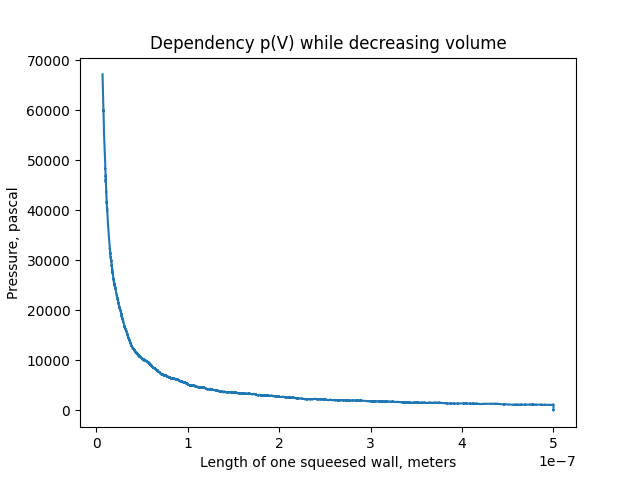
\includegraphics[scale=0.3]{pv.png}
  \end{itemize}
\end{frame}

\begin{frame}{Experiment}
  \begin{itemize}    
    \item Теперь будем постепенно нагревать молекулы. Ожидается, что получится линейная зависимость: $p = C\cdot T$. Действительно, после выравнивания давления и начала нагрева вырисовывается линейная зависимость.
    
    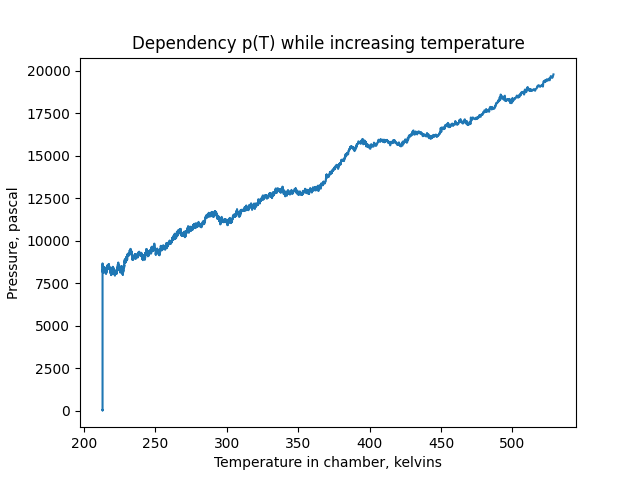
\includegraphics[scale=0.3]{pt.png}
  \end{itemize}
\end{frame}

\begin{frame}{Experiment}
  Также хотелось бы рассказать о проведённом нами эксперименте:
  \begin{itemize}
    \item<1-> В одной из стенок была проделана квадратная дыра.
    \item<2-> Зафиксировали количество горячих частиц до открытия дыры
    \item<3-> Открыли отверстие и подождали небольшое время (Около минуты)
    \item<4-> Оказалось, что в начале температура уменьшается очень резко, вероятно всего из-за быстрых молекул, вероятность вылета которых существенно больше.
  \end{itemize}
\end{frame}

\begin{frame}{Graph}
  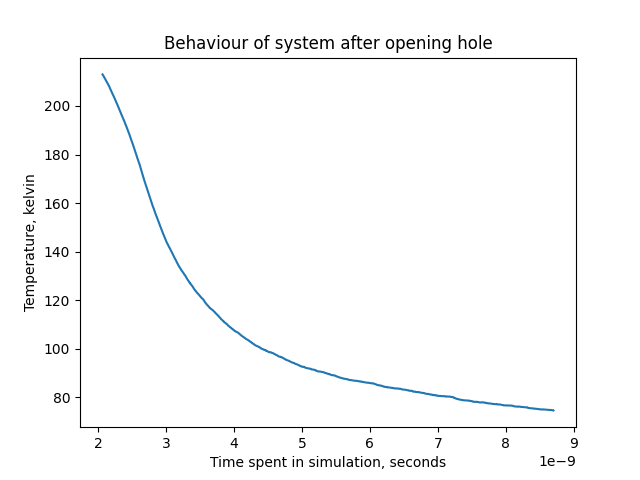
\includegraphics[scale=0.5]{holettime.png}
\end{frame}

\begin{frame}{Experiment}
  Смотреть за молекулами одного газа конечно здорово, но есть эксперимент поинтереснее -- диффузия.

  \begin{figure}
    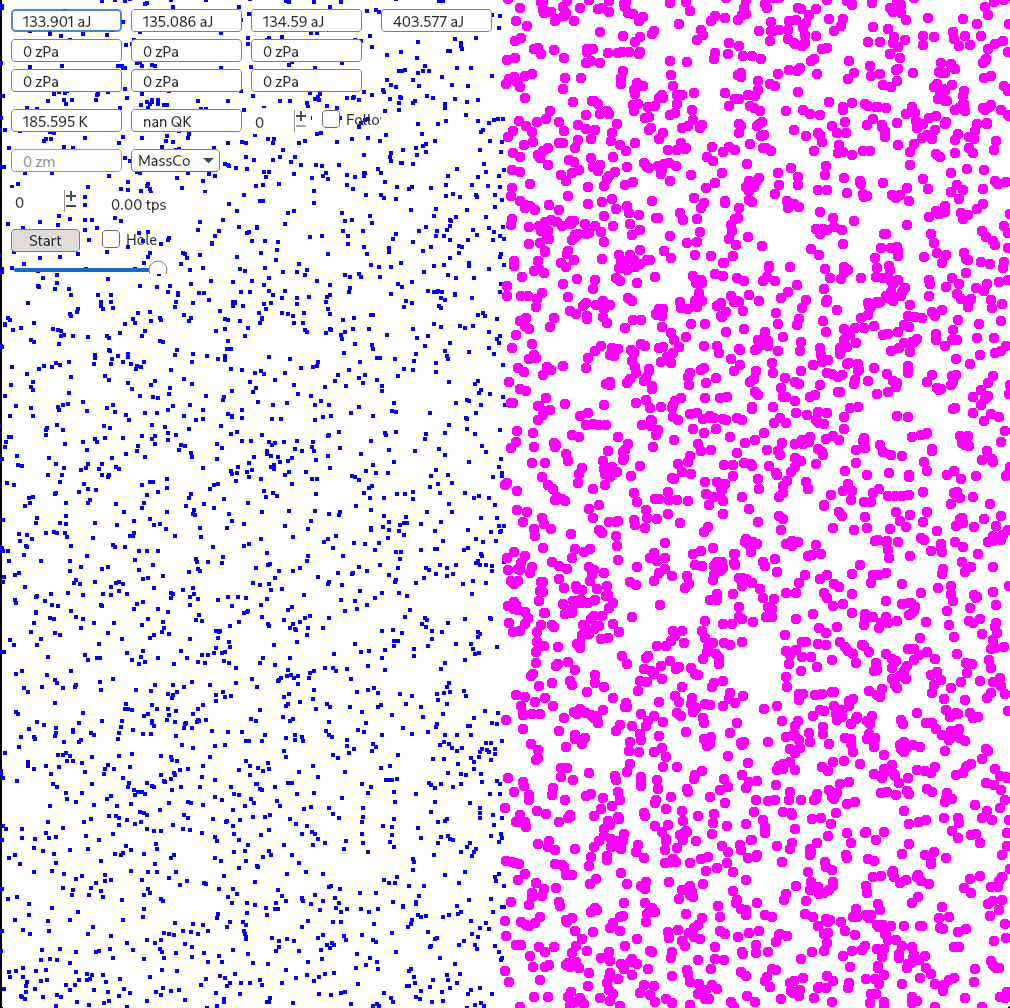
\includegraphics[scale=0.11]{diffusion.png}
    \caption{Гелий и ксенон}
  \end{figure}
\end{frame}

\begin{frame}{Experiment}
  Как мы показывали ранее, диффузия происходит. Но есть ли какие-то способы проверить, насколько корректно? 
  
  \pause[2]
  Да! Мы можем посчитать коэффициент диффузии с помощью закона Фика для какой-то из стенок камеры:
  \[
    \frac{\nu}{S\cdot \Delta t} = \frac{\Delta P}{l}D 
  \]
  где $\frac{\nu}{\Delta t}$ -- количество вещества, столкнувшегося со стенкой за время $\Delta t$, $S$ -- площадь стенки, $\Delta P$ -- изменение давления за это время, $l = \frac{V}{S}$, а $D$ -- коэффициент, который хотим найти.
\end{frame}

\begin{frame}{Experiment}
  Реализовав все необходимые функции, получили $D \sim 2 \cdot 10^{-7}$ $\text{м}^2$/с. Но что это за попугаи? Реально ли это?

  \pause[2]
  В начале обратимся к Википедии -- в нормальных условиях для молекул газов коэффициент имеет порядок $10^{-5}$. Но наши условия совсем ненормальные -- температура $185.6$ К, а давление $1.6$ МПа. 

  Для $D$ имеем зависимость $\sim \frac{T^{3/2}}{P}$, подставив условия эксперимента получим, что наш коэффициент должен быть в $32$ раза меньше значения из Википедии. Это около $3.125 \cdot 10^{-7}$, мы близко!
\end{frame}

\begin{frame}{Experiment}
  Но что если хотим посчитать коэффициент как-то по-другому, используя нашу модель? Можно ли это сделать? 
  
  \pause[2]
  Существуют коэффициенты самодиффузии для каждого из газов в отдельности. Чтобы получить уже искомый коэффициент диффузии воспользуемся формулой
  \[
    \frac{D_1n_1 + D_2n_2}{n_1 + n_2}
  \]
  где $n_i$ -- концентрация соответствующего газа. В нашем случае концентрации равны, поэтому просто возьмём полусумму.
\end{frame}

\begin{frame}{Experiment}
  Но откуда взять эти коэффициенты самодиффузии? Существует формула, использующая длину свободного пробега, а также среднюю скорость молекул. Мы их знаем!
  \[
    D_{self} = \frac{1}{3}\lambda\overline{v}
  \]
  Запустив симуляцию для каждого из газов поотдельности получим значения $1.7 \cdot 10^{-7}$ и $9.35 \cdot 10^{-7}$ для ксенона и гелия соответственно.
\end{frame}

\begin{frame}{Experiment}
  Получили альтернативное значение коэффицента диффузии $\sim 5.5 \cdot 10^{-7}$. Разница c изначальным значением $2 \cdot 10^{-7}$ в $2.75$ раза. 
  
  Многовато. Почему?

  Если снова посмотреть на формулу коэффициента самодиффузии в учебнике, то увидим, что это всего лишь оценка, имеющая погрешность в $50 \%$, а если ещё вспомнить, что $\Delta t$ у нас не такое уж и маленькая, то полученная разность становится объяснимой.
\end{frame}

\section{Results}

\begin{frame}
  \begin{itemize}
    \item<1-> Смоделировали идеальный газ
    \item<2-> Собрали множество метрик
    \item<3-> Проверили выполнение основного уравнение для идеального газа
    \item<4-> Проверили занимательный эксперимент с отверстием
    \item<5-> Смоделировали диффузию двух газов и посчитали коэффициент диффузии разными способами
  \end{itemize}
\end{frame}

\end{document}
